Going a step back and asking why genomes are studied, many times the answer is
that one wants to understand the function of genes and proteins. The genome is
made up of long strands of deoxyribonucleic acid (DNA). It contains the
necessary instructions to create and maintain cells.  Proteins are produced
according to information on the DNA in a two-step process: during
\emph{transcription}, messenger ribonucleic acid (\nomenclature{mRNA}{Messenger
ribonucleic acid}) is synthetisized. In the second step, \emph{translation}, the
mRNA is used by specialized organelles, namely ribosomes, to synthetisize
proteins from amino acids. In eukaryotes, this process includes \emph{splicing},
during which non-coding regions, so-called \emph{introns} are removed from the
mRNA. In bacteria and archaea, the mRNA requires typically no further processing
before translation. The resulting molecule contains only \emph{exons}, coding
regions of the genome that are relevant for translation. The ratio of exons to
introns varies across organisms; \eg, the human genome consists of only 1.1\% to
1.4\% exons and 24.4\% to 37.8\% introns, the rest is intergenic DNA
\citep{venter2001}. That means that in eukaryotes, the majority of the genome
does not code for proteins, and the functional analysis of the genes in an
eukaryote genome requires screening the nucleotide sequence data for those
non-coding regions.

The study of \emph{transcriptomes} circumvents these problems. A transcriptome
is the collection of all transcripts in a tissue sample at the time of RNA
preservation.  Transcriptomes are frequently used in phylogenetics and
phylogenomics to reconstruct species trees based on hundreds of
genes\footnote{The \nomenclature{1KITE}{1,000 insect transcriptome evolution}
project (1K Insect Transcriptome Evolution, \url{http://1kite.org}) aims to
sequence the transcriptomes of 1,000 insect species and infer a robust backbone
tree of insects. Preliminary analyses were performed on a supermatrix of 1,478
genes.}.  The combination of low-cost next-generation sequencing and the
intron-free nature of transcriptomes allow access to a high proportion of
protein coding genes per sequenced mega-base pair at a fraction of the cost for
sequencing the corresponding genome.

Next-generation transcriptome sequencing technologies achieve their high
throughput by massively parallelizing the sequencing process. They cannot
sequence whole genomes in a single run, but produce a large number of so-called
\emph{reads}, short nucleotide sequences (20 to 1,000
\nomenclature{bp}{basepair(s)} in length, depending on the technology used).
These fragments must be \emph{assembled} to form so-called \emph{contigs},
contiguous sequences of nucleotides that most closely resembles the nucleotide
sequence present in the sequenced specimen. The assembly process is a
computationally complex problem that has not yet been solved to perfection.
Reviews of different strategies have been written by, \eg, \citet{zhang2011}.
The assembled data may be redundant due to, \eg, alternative splicing products
\citep{black2003} or multiple, non-overlapping sequencing of C-terminus and
N-terminus (the two ends of a DNA strand or gene).  Most assembly software
cannot detect these issues reliably \citep{haiminen2011}. 

In addition to the processes explained above, next-generation transcriptome
sequencing and assembly output sequence data are not only fragmented and
possibly redundant (overlapping), but most importantly they are
\emph{incomplete} because not all genes may have been expressed at the time of
preservation. Due to this inherent incompleteness of transcriptomes, orthology
prediction approaches that are used on fully sequenced and annotated genomes
cannot be used.

\begin{figure}[t]
	\centering
	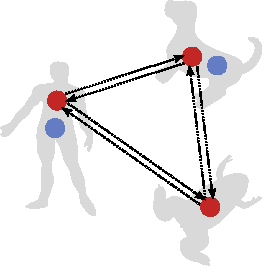
\includegraphics[width=0.4\textwidth]{img/triangulation-bbh.pdf}
	\caption[Bidirectional best hit (BBH) triangulation]{
		Bidirectional best hit (BBH) triangulation. To identify genes as orthologous
		in the presence of potential gene loss or incomplete data, they must be BBH
		in three species.  In this example, the red gene fulfills this criterion.
		The blue gene cannot be unambiguously identified as orthologous, as it is
		not present in the frog and paralogy is possible (compare to
		\autoref{fig:graph-based-strat}).  Graphic modified from
		\citet{altenhoff2012}.
	}
	\label{fig:triangulation-bbh}
\end{figure}


When performing a bidirectional search on a fully sequenced and annotated
complete genome as described above, it can happen that two genes that are
identified as BBH are paralogs because the corresponding orthologs have been
lost in both investigated species. This situation is called \emph{differential
gene loss}\cite{altenhoff2012} and best solved using a tree-based approach. In
the face of the aforementioned difficulties of a tree-based strategy, some
graph-based algorithms implement \emph{triangulation}
(\autoref{fig:triangulation-bbh}): to identify two genes as orthologous, they
must be BBH not only in two, but in three species. The third gene functions as
possible ``witness of non-orthology'' \citep{dessimoz2006}. A triangulation
strategy can also be applied to orthology prediction in transcriptomic data, the
incompleteness of which may be seen as a similar situation as potential gene
loss in fully sequenced and annotated genomes. This approach has been
implemented in \hamstr \citep{ebersberger2009}, which I will describe in the
following section.
